\documentclass[conference]{IEEEtran}

\usepackage{cite}
\usepackage{amsmath,amssymb}
\usepackage{graphicx}
\usepackage[caption=false,font=footnotesize]{subfig}
\usepackage{algorithm}
\usepackage{algpseudocode}
\usepackage{booktabs}
\usepackage{xcolor}
\usepackage{url}
\usepackage[colorlinks=true,urlcolor=blue,linkcolor=black,citecolor=black]{hyperref}
\usepackage{listings}
\lstset{basicstyle=\ttfamily\tiny,breaklines=true,breakatwhitespace=false,
  columns=fullflexible,keepspaces=true,frame=single}

\graphicspath{{greedy/figures/}{figures/}}

\newtheorem{lemma}{Lemma}
\newtheorem{theorem}{Theorem}

\begin{document}

\title{Minimum-Cable Campus Networks: A Greedy Minimum Spanning Tree Approach}

\author{
\IEEEauthorblockN{Sridhar Kumar}
\IEEEauthorblockA{\textit{Department of Computer Science}\\
\textit{University of Florida}\\
Gainesville, FL, USA\\
f.sridharkumar@ufl.edu}
\and
\IEEEauthorblockN{Daen P Khan}
\IEEEauthorblockA{\textit{Department of Computer Science}\\
\textit{University of Florida}\\
Gainesville, FL, USA\\
dpatan@ufl.edu}
}

\maketitle

\begin{abstract}
Campus telecommunications planning requires a connected backbone between
buildings, but candidate routes differ in cable length. We model this planning
problem as a weighted undirected graph and seek a connected set of routes with
minimum total length. Kruskal's greedy algorithm sorts routes by length and
accepts a route only when it joins two currently disconnected components. A
cut-property exchange argument proves that every accepted route is safe and
that the final network is a minimum spanning tree. With a disjoint-set data
structure, the implementation runs in $O(E\log E)$ time and uses $O(E+V)$
space. Tests and a reproducible experiment over 28 connected synthetic graph
families support the predicted growth.
\end{abstract}

\begin{IEEEkeywords}
greedy algorithms, minimum spanning tree, Kruskal's algorithm, campus
cabling, graph optimization
\end{IEEEkeywords}

%======================================================================
\section{Introduction}
%======================================================================

Campus network planners must connect buildings through feasible pathways such
as conduit, utility tunnels, and approved interbuilding backbone routes. Each
possible route has a measured cable length and installation plan. The base
planning question is to connect every building while minimizing the total
amount of cable installed. Campus infrastructure standards describe these
pathways as a distinct engineering concern~\cite{yale2025infrastructure}.

This paper studies the base minimum-cable problem as a greedy algorithm
application. The buildings and feasible routes form a weighted graph, and the
desired network is a minimum spanning tree (MST). Kruskal's algorithm makes a
local choice: among the remaining routes, choose the shortest route that does
not create a cycle. The cut property shows why this local rule preserves a
globally optimal solution.

Our contributions are:
\begin{itemize}
  \item a graph abstraction of minimum-cable campus backbone planning;
  \item a formal Kruskal algorithm using a disjoint-set forest;
  \item a cut-property exchange proof of optimality;
  \item an $O(E\log E)$ running-time analysis; and
  \item an implementation, correctness test suite, and timing experiment.
\end{itemize}

%======================================================================
\section{Related Work and Domain Context}
%======================================================================

Minimum spanning trees are used when a set of weighted links must connect all
vertices at minimum total weight. Kruskal's algorithm is a standard greedy
solution and uses disjoint sets to test whether a candidate edge joins
different components~\cite{cormen2009introduction}. The engineering motivation
here comes from campus outside-plant telecommunications. Real projects can
also require redundancy, route diversity, capacity limits, and construction
costs~\cite{yale2025infrastructure}. Those requirements are outside the base
optimization model so that the greedy structure can be analyzed directly.

%======================================================================
\section{Problem Formulation}
%======================================================================

\subsection{Real-World Problem}

A campus has a collection of buildings and a survey of permitted pathways
between pairs of buildings. For each pathway, the survey records the cable
length needed to connect its endpoints. Every building must be able to reach
every other building through the installed network, possibly through
intermediate buildings, while the total installed cable is minimized.

The model assumes that every supplied route is physically feasible, lengths
already reflect the selected pathway, and a building may forward traffic. It
does not include backup links, link capacity, excavation cost, or a requirement
for two physically diverse paths. Those constraints can lead to richer network
design problems, but they are not part of this report's objective.

\subsection{Mathematical Abstraction}

Let $G=(V,E)$ be a connected undirected graph. Each vertex $v\in V$ is a
building. Each edge $e=\{u,v\}\in E$ is an approved route, with positive
weight $w(e)$ equal to its required cable length. We seek a subset $T\subseteq
E$ such that $(V,T)$ is connected and
\begin{equation}
  W(T)=\sum_{e\in T} w(e)
\end{equation}
is minimum. Any connected solution containing a cycle can remove one cycle
edge and remain connected. Since all weights are positive, an optimal solution
is acyclic and therefore contains exactly $|V|-1$ routes. The problem is thus
the minimum spanning tree problem.

\medskip
\noindent\textbf{Problem (Minimum-Cable Network).}
\emph{Input:} a connected weighted graph $G=(V,E)$.\\
\emph{Output:} a spanning tree $T$ minimizing $W(T)$.\\
\emph{Cost:} total route length, with running time measured separately.

%======================================================================
\section{Greedy Algorithm}
%======================================================================

\subsection{Strategy}

Kruskal's algorithm sorts all routes in nondecreasing order of length. It
starts with each building as its own component. A route is installed when its
endpoints are in different components; the two components are then merged. A
route whose endpoints are already connected would create a cycle and is
skipped. The algorithm stops after $|V|-1$ routes have been accepted.

\begin{algorithm}[t]
\caption{Kruskal minimum-cable network}
\label{alg:kruskal}
\begin{algorithmic}[1]
\Require connected graph $G=(V,E)$ with positive route lengths $w$
\Ensure minimum-length set of routes connecting all buildings
\State $T\gets\emptyset$
\ForAll{$v\in V$}
  \State \Call{MakeSet}{$v$}
\EndFor
\State sort $E$ by nondecreasing $w(e)$
\ForAll{$e=\{u,v\}\in E$ in sorted order}
  \If{$\Call{Find}{u}\ne\Call{Find}{v}$}
    \State $T\gets T\cup\{e\}$
    \State \Call{Union}{$u,v$}
    \If{$|T|=|V|-1$}
      \State \Return $T$
    \EndIf
  \EndIf
\EndFor
\State report that the route graph is disconnected
\end{algorithmic}
\end{algorithm}

In domain terms, the planning team considers the shortest available cable
route first. It installs that route when it connects two groups of buildings
that cannot yet communicate. Routes internal to one existing group are not
needed for the minimum-cable backbone because they only create cycles.

\subsection{Worked Example}

Suppose four buildings have feasible routes of lengths $1$, $2$, $3$, $4$,
and $5$ meters, where the first three selected routes connect all four
buildings. Kruskal accepts the $1$-meter route, then the $2$-meter route, and
then the $3$-meter route. If the $4$-meter route would join buildings already
connected by those choices, it is skipped. The resulting tree has total length
$1+2+3=6$ meters and connects every building with no cycle.

\subsection{Implementation Notes}

The C++17 implementation stores each route as its two endpoints, a signed
64-bit length, and its input order. It validates positive lengths and endpoint
ranges before sorting. Ties are deterministic: route length, normalized
endpoints, and input order are used as tie breakers. Path compression and
union by rank implement the disjoint-set forest. The implementation detects
disconnected input and checks for signed 64-bit overflow when accumulating the
total length.

%======================================================================
\section{Complexity Analysis}
%======================================================================

Sorting $E$ routes costs $O(E\log E)$. With path compression and union by
rank, all disjoint-set operations over the route scan cost
$O(E\alpha(V))$, where $\alpha$ is the inverse Ackermann function
\cite{cormen2009introduction}. Therefore,
\begin{equation}
  T(V,E)=O(E\log E).
\end{equation}
The route list, selected tree, and disjoint-set arrays use $O(E+V)$ space. If
every pair of buildings is a candidate route, $E=\Theta(V^2)$ and the bound
becomes $O(V^2\log V)$.

%======================================================================
\section{Proof of Correctness}
%======================================================================

\begin{lemma}[Safe greedy route]\label{lem:safe}
Let $A$ be the set of routes already selected by Kruskal, and suppose some MST
$M$ contains $A$. If the next accepted route $e$ joins two different
components of $(V,A)$, then some MST contains $A\cup\{e\}$.
\end{lemma}

\begin{IEEEproof}
Let $C$ be the component of $(V,A)$ containing one endpoint of $e$. The
other endpoint lies outside $C$, so $e$ crosses the cut $(C,V\setminus C)$.
At the time $e$ is selected, it is a lightest eligible route crossing this
cut: a lighter route crossing the cut would also join different components and
would have appeared earlier in the sorted scan.

If $e\in M$, the claim is immediate. Otherwise, adding $e$ to the tree $M$
creates one cycle. That cycle contains an edge $f$ crossing the cut. No edge
of $A$ crosses between two components of $(V,A)$, so $f\notin A$. Since
$e$ is a lightest eligible crossing route, $w(e)\le w(f)$. Replacing $f$ by
$e$ gives $M'=M-\{f\}+\{e\}$, a spanning tree with no greater weight. The
minimality of $M$ implies that $M'$ is also an MST, and it contains
$A\cup\{e\}$.
\end{IEEEproof}

\begin{theorem}\label{thm:correct}
Algorithm~\ref{alg:kruskal} returns a minimum-length connected cable network
for every connected input graph.
\end{theorem}

\begin{IEEEproof}
Initially $A=\emptyset$, which is contained in an MST. By Lemma~\ref{lem:safe},
after each accepted route there remains an MST containing all routes selected
so far. Because the input graph is connected, the algorithm eventually accepts
$|V|-1$ routes. The accepted routes are acyclic because a route is accepted
only when it joins distinct components, so they form a spanning tree. An MST
contains all of this tree's $|V|-1$ routes and has the same number of edges;
therefore the selected tree itself is an MST and has minimum total cable
length.
\end{IEEEproof}

%======================================================================
\section{Experimental Validation}
%======================================================================

\begin{figure*}[!t]
\centering
\subfloat[Runtime and $E\log E$ fit.]{%
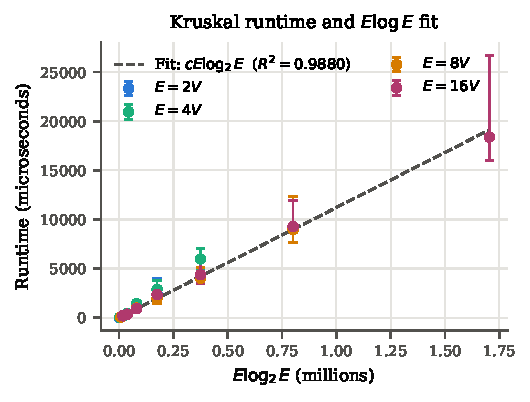
\includegraphics[width=0.48\textwidth]{fig1_runtime_fit.pdf}}
\hfill
\subfloat[Runtime normalized by $E\log E$.]{%
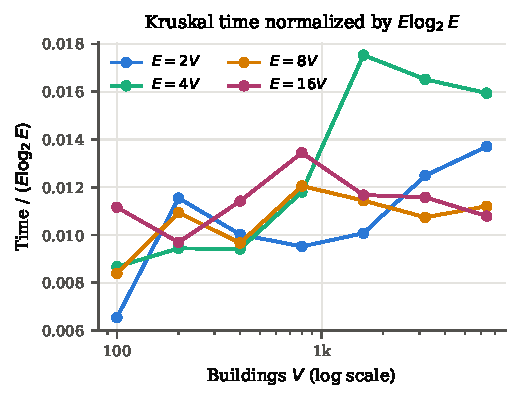
\includegraphics[width=0.48\textwidth]{fig2_normalized_time.pdf}}
\\[4pt]
\subfloat[Kruskal versus Prim on $E=8V$.]{%
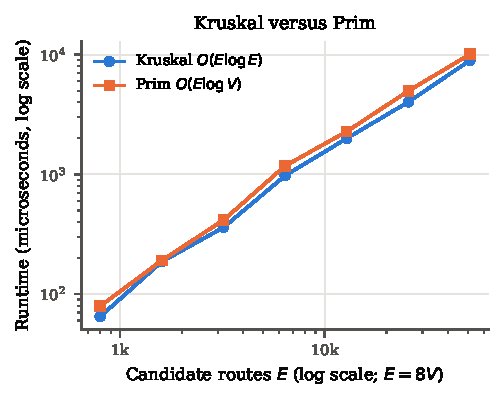
\includegraphics[width=0.48\textwidth]{fig3_baselines.pdf}}
\hfill
\subfloat[Scaling across route densities.]{%
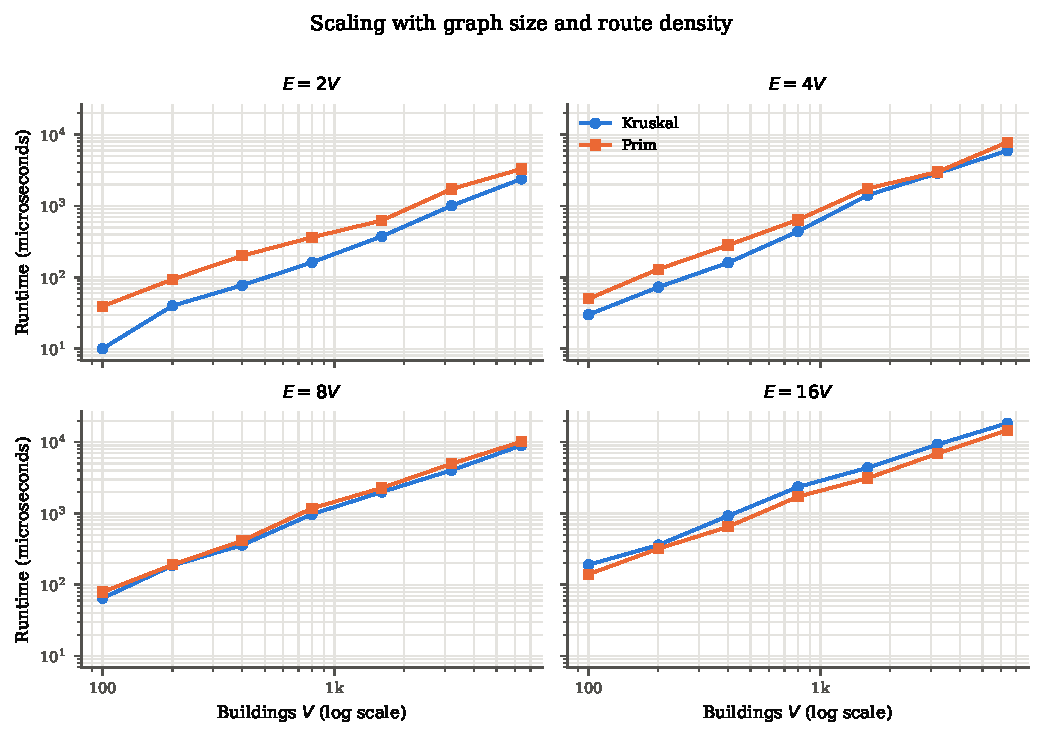
\includegraphics[width=0.48\textwidth]{fig4_density_scaling.pdf}}
\caption{Experimental results for Kruskal's minimum-cable algorithm on 28
connected synthetic graph families.}
\label{fig:greedy-results}
\end{figure*}

\subsection{Correctness Testing}

The test suite covers the six-route example, malformed input, disconnected
graphs, parallel routes, equal weights, a single building, large integer
weights, and 64-bit overflow. Small graphs are compared with exhaustive
enumeration of all candidate spanning trees. A seeded 800-building graph with
16,000 routes is checked against an independent Prim implementation. A
5,000-building sparse graph with a known optimum provides an additional stress
case. All eleven test groups are intended to check both the CLI output and the
selected tree structure.

\subsection{Synthetic Graphs and Setup}

The benchmark generates connected random graphs with
$V\in\{100,200,400,800,1600,3200,6400\}$ and
$E\in\{2V,4V,8V,16V\}$. A random spanning chain is inserted first, so every
generated graph is connected; remaining routes are sampled without duplicate
undirected endpoints. Route lengths are positive random integers. Graph
generation occurs outside the timer. Each of the 28 graph families uses a
fixed seed and seven trials. Short runs are repeated inside each trial, and
the reported time is the average duration of one algorithm call. The same
graphs are timed with an independent Prim implementation, producing 392
algorithm observations in the CSV (196 per algorithm).

The experiment was compiled with MinGW GCC 6.3.0 using
\texttt{-std=c++17 -O2 -Wall -Wextra -pedantic} on Windows. Processor and
memory details should be recorded when the final submission run is performed.

\subsection{Results}

The smallest Kruskal case, $V=100$ and $E=200$, had a median runtime of
$10.00\,\mu$s. At the largest graph, $V=6400$ and $E=102400$, the median
Kruskal time was $18391.33\,\mu$s and the median Prim time was
$14680.33\,\mu$s. A line proportional to $E\log_2E$ fitted through the
origin gave $R^2=0.98804$ across the 28 Kruskal median points (Fig.~\ref{fig:greedy-results}a).
The normalized values in Fig.~\ref{fig:greedy-results}b remain comparable
across route densities. Prim was between 1.02 and 1.24 times the Kruskal time
at $E=8V$, with the ratio varying by graph size (Fig.~\ref{fig:greedy-results}c).
The density panels in Fig.~\ref{fig:greedy-results}d show that both methods
slow as candidate routes become denser. These measurements agree with the
derived $O(E\log E)$ upper bound; they do not replace the correctness proof or
establish an asymptotic bound by themselves.

\begin{table}[t]
\centering
\caption{Median Kruskal runtime in microseconds}
\label{tab:kruskal-times}
\scriptsize
\begin{tabular}{@{}rrrrr@{}}
\toprule
$V$ & $E=2V$ & $E=4V$ & $E=8V$ & $E=16V$ \\
\midrule
100  & 10.00 & 29.98 & 64.75 & 190.09 \\
200  & 39.92 & 72.83 & 186.21 & 361.14 \\
400  & 77.32 & 160.32 & 360.08 & 924.04 \\
800  & 162.12 & 439.68 & 975.16 & 2347.36 \\
1600 & 375.38 & 1418.50 & 1998.00 & 4376.38 \\
3200 & 1010.12 & 2884.75 & 4026.50 & 9274.25 \\
6400 & 2393.33 & 5975.00 & 8973.67 & 18391.33 \\
\bottomrule
\end{tabular}
\end{table}

\begin{table}[t]
\centering
\caption{Median Prim runtime in microseconds}
\label{tab:prim-times}
\scriptsize
\begin{tabular}{@{}rrrrr@{}}
\toprule
$V$ & $E=2V$ & $E=4V$ & $E=8V$ & $E=16V$ \\
\midrule
100  & 39.36 & 50.06 & 79.17 & 140.41 \\
200  & 93.26 & 129.98 & 190.77 & 320.66 \\
400  & 200.60 & 283.08 & 414.52 & 650.08 \\
800  & 363.56 & 639.68 & 1176.96 & 1717.56 \\
1600 & 626.62 & 1758.50 & 2282.88 & 3125.12 \\
3200 & 1729.50 & 3000.12 & 4972.62 & 6907.50 \\
6400 & 3307.33 & 7845.00 & 10111.33 & 14680.33 \\
\bottomrule
\end{tabular}
\end{table}

%======================================================================
\section{Discussion and Limitations}
%======================================================================

Kruskal's method is appropriate when the planning objective is the sum of
positive route lengths and every building only needs to be connected. Its
greedy decisions are irrevocable, but the cut-property proof guarantees that
each decision can be extended to an optimal tree. The disjoint-set data
structure keeps cycle checks efficient even when the route list is large.

The model does not guarantee network resilience. A real campus backbone may
need two independent paths, capacity guarantees, existing-duct constraints,
construction costs, or protection against a single route failure. Those goals
require a more expressive network design model. The experiment also uses
synthetic graphs and measures algorithm time rather than construction time;
the results validate implementation growth, not real project cost.

%======================================================================
\section{Conclusion}
%======================================================================

We formulated minimum-cable campus backbone planning as a weighted graph
problem and solved it with Kruskal's greedy algorithm. The cut-property
exchange argument proves that the selected routes form an MST. The C++17
implementation runs in $O(E\log E)$ time, handles invalid and disconnected
inputs, and was tested against exhaustive and Prim-based references. A fixed
seed experiment over 28 connected graph families produced timing growth
consistent with $E\log E$.

%======================================================================
\begin{thebibliography}{9}

\bibitem{yale2025infrastructure}
Yale University, ``IT infrastructure design guidelines and performance
standards,'' sec. 1.16, Interbuilding Backbone Pathways, 2025. [Online].
Available: \href{https://facilities.yale.edu/sites/default/files/files/Design\%20Standards/IT\%20Infrastructure\%20Design\%20Guidelines\%20and\%20Performance\%20Standards_Rev1_5.pdf}{Yale IT infrastructure design guidelines}.

\bibitem{cormen2009introduction}
T. H. Cormen, C. E. Leiserson, R. L. Rivest, and C. Stein,
\emph{Introduction to Algorithms}, 3rd ed. Cambridge, MA, USA: MIT Press,
2009.

\end{thebibliography}

\appendices

\section{Runtime Validation Code}

The following source files generate the connected test graphs, run Kruskal's
algorithm and the Prim baseline, measure repeated trials, and write the CSV
data used for the experimental figures.  The implementation files included
below are the algorithm code called by the benchmark.

\lstinputlisting[language=C++,caption={Greedy benchmark harness}]{greedy/experiments/benchmark.cpp}
\lstinputlisting[language=C++,caption={Minimum-spanning-tree interface}]{greedy/src/mst.hpp}
\lstinputlisting[language=C++,caption={Minimum-spanning-tree implementation}]{greedy/src/mst.cpp}

\section{LLM Usage}

We used Chat GPT Codex (model GPT-5.6-Luna high, by OpenAI),
accessed using the terminal client for Windows.
It was used to tackle the correctness of the problem, implement
some of the C++ code and plotting script, run the experiments,
generate the figures, draft this report in LaTeX.

\begin{enumerate}
\item \textbf{Prompt:} \emph{Connecting buildings with the least amount of cable using MST. This is the topic which we have decided. As you can see this is a greedy type problem.}
\item \textbf{Prompt:} \emph{Model the campus minimum-cable problem as a weighted undirected graph. Define the vertices, edges, weights, feasible output, and objective precisely.}
\item \textbf{Prompt:} \emph{Explain why a minimum spanning tree is the correct abstraction and compare Kruskal and Prim. Choose the most appropriate greedy algorithm for this report and justify the choice.}
\item \textbf{Prompt:} \emph{Write clear pseudocode for Kruskal's algorithm using a disjoint-set data structure, including initialization, sorting, cycle checks, termination, and disconnected-input handling.}
\item \textbf{Prompt:} \emph{Explain path compression and union by rank in the disjoint-set forest, and describe how they affect the running time of Kruskal's algorithm.}
\item \textbf{Prompt:} \emph{Derive the time and space complexity of Kruskal's algorithm in terms of vertices and edges. Explain why sorting gives the final $O(E\log E)$ bound.}
\item \textbf{Prompt:} \emph{Give a rigorous cut-property or exchange-argument proof that every edge accepted by Kruskal can be part of an MST, and then use it to prove the full algorithm correct.}
\item \textbf{Prompt:} \emph{Explain Kruskal's algorithm in campus-networking language while preserving the connection between short cable routes, connected components, cycles, and minimum total cable.}
\item \textbf{Prompt:} \emph{Implement the campus-network MST algorithm in portable C++17 with deterministic tie handling, input validation, disconnected-graph detection, and safe total-length accumulation.}
\item \textbf{Prompt:} \emph{Design tests for the MST implementation covering normal graphs, a single vertex, equal weights, parallel routes, disconnected inputs, malformed endpoints, large weights, overflow, and comparison with an independent reference.}
\item \textbf{Prompt:} \emph{Design a reproducible timing experiment for Kruskal's algorithm using fixed seeds, connected synthetic graphs, multiple values of $V$ and $E$, repeated trials, warm-up/repetition handling, and CSV output.}
\item \textbf{Prompt:} \emph{Add an independent Prim implementation as a baseline, verify that Kruskal and Prim produce the same MST total, and record both runtimes without including graph generation in the timed region.}
\item \textbf{Prompt:} \emph{Create publication-quality plots showing runtime versus $E\log E$, normalized runtime, Kruskal versus Prim, and scaling across graph densities. Also generate a concise numerical summary.}
\item \textbf{Prompt:} \emph{Interpret the benchmark results cautiously: explain how the graphs support the predicted $O(E\log E)$ growth, distinguish empirical evidence from a proof, and state the experiment's limitations.}
\end{enumerate}

\section*{Code Availability}

The implementation, tests, benchmark, raw CSV results, plotting script, and
generated figures are available in the repository under \texttt{greedy/}.
The complete code repository is available at
\href{https://github.com/Sridhar-97k/AOA_Project1.git}{github.com/Sridhar-97k/AOA\_Project1}.
From the repository root, compile the report with
\texttt{latexmk -pdf greedy/greedy\_report.tex}. Build and experiment
commands are documented in \texttt{greedy/README.md}.

\end{document}
